\chapter{Diseño e implementación} % Main chapter title

\label{Chapter3} % Change X to a consecutive number; for referencing this chapter elsewhere, use \ref{ChapterX}


Este capítulo explica los componentes del sistema seleccionados y la descripción detallada de cada módulo de hardware y software desarrollados en el trabajo. Utilizando las definiciones y criterios descritos en capítulos anteriores, se comprende el diseño final del prototipo.

%----------------------------------------------------------------------------------------
%	SECTION 1
%----------------------------------------------------------------------------------------
\section{Diseño e implementación general del sistema}

El diseño e implementación general del sistema se subdividió en 3 partes: 

\begin{enumerate}
    \item Diseño e implementación del hardware.
    \item Diseño e implementación del firmware.
    \item Diseño e implementación de la interfaz web.
\end{enumerate}

A continuación, se describen cada una de estas partes.

%----------------------------------------------------------------------------------------
%	SECTION 2
%----------------------------------------------------------------------------------------
\section{Diseño e implementación de hardware}
\label{sec:dis_impl_hardware}

En esta sección, se describen las consideraciones de diseño del hardware del sistema. 

\subsection{Diseño del Hardware}

En la figura~\ref{fig:Arq_harware} se presenta la arquitectura del hardware desarrollado. Se incluyen todos los componentes descritos en las secciones anteriores. El sistema cuenta con 3 antenas correspondientes a la comunicación GNSS, 4G y Wi-Fi. 

Como parte de la interfaz humano-máquina, se cuenta con una pantalla LCD de 16x2, un botón para la indicación manual de estado ocupado/desocupado y dos pilotos que permiten visualizar el estado de ocupación actual. 

En el diagrama se pueden ver los protocolos de comunicación entre módulos, entre los que se destacan:

\begin{itemize}
    \item El protocolo UART para la comunicación entre el módulo 4G SIM A7670SA por el puerto UART 0 y el módulo  GNSS Quectel L76 por el puerto UART 1. 
    \item El protocolo I2C para la comunicación con la pantalla LCD. 
\end{itemize}

Se presenta una fuente de alimentación correspondiente a una batería de 12 VDC. Debido a que los componentes del sistema operan con tensiones diferentes, se hizo necesaria la implementación de circuitos adicionales. En el diagrama, estos circuitos se denominan <<Fuente>>. Estos suplen 2 niveles de tensión distintos: 
\begin{itemize}
    \item 3,3 VDC para el Quectel L76.
    \item 5 VDC para la ESP32, el módulo SIM A7670SA y la pantalla LCD.
\end{itemize}



\begin{figure}[htbp]
	\centering
	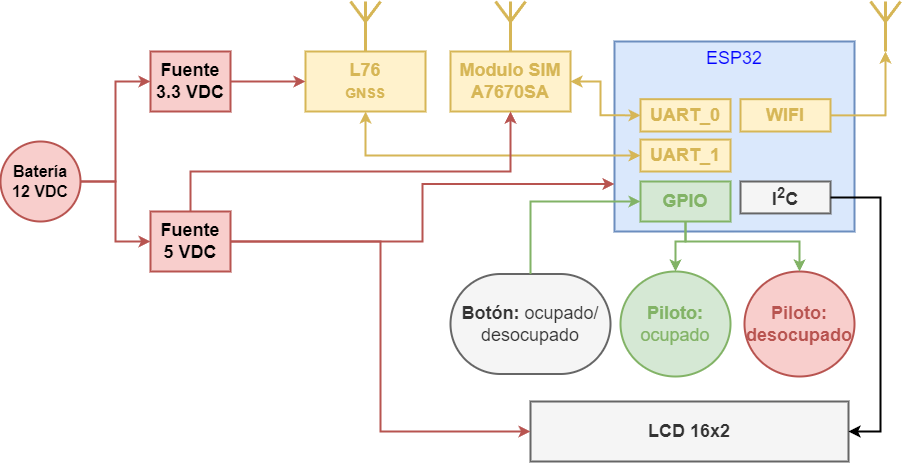
\includegraphics[width=1\textwidth]{./Figures/arquitectura_hardware_sistema.png}
	\caption{Arquitectura del hardware desarrollado.}
	\label{fig:Arq_harware}
\end{figure}



\subsection{Implementación del Hardware}

En la etapa de implementación del hardware, se trabajó en 2 placas de circuito impreso. 

\begin{enumerate}
    \item Placa base del sistema.
    \item Adaptador para el módulo Quectel L76.
\end{enumerate}



\subsubsection{Placa base del sistema}

La placa base se encargará de interconectar los módulos y periféricos principales del sistema. Por lo tanto, en el apéndice~\ref{AppendixA}, se presenta el circuito esquemático correspondiente a esta implementación. En esta se empleó el regulador MIC29302WU, con una configuración de ajuste por defecto en 5 VDC, para la alimentación de la ESP32, del módulo SIM A7670SA, la placa adaptador para el módulo Quectel L76 y la Pantalla LCD. En la figura~\ref{fig:placa_base_2d} se puede apreciar el diseño final del PCB en un modelo de dos dimensiones. Además, en la figura~\ref{fig:placa_base_3d} se observa el modelo en tres dimensiones. 

Los componentes U1, U2 y H3, corresponden a las ranuras donde se conectan la ESP32 DevKit V4, el adaptador para el módulo Quectel L76, y el módulo SIM A7670SA. Las terminales marcadas con CN6 y CN7 permiten la conexión de los pilotos que indican la ocupación de la cava. Las terminales CN4 y CN5 corresponden a las conexiones de los botones de que dispondrá el operario de la cava para la indicación de la ocupación. Por otro lado, las terminales CN2 y CN3 corresponden a la interfaz I2C y la alimentación de la pantalla LCD, respectivamente. La bornera CN1 corresponde a la entrada de alimentación del sistema. Finalmente, las terminales CN9 y CN11 externalizan los pines GPI 34 y GPI 35, y GPIO 5 y GPIO 18 de la ESP32, respectivamente; esto para facilitar, en una etapa posterior, la agregación de nuevas funcionalidades. 

\begin{figure}[htbp]
	\centering
	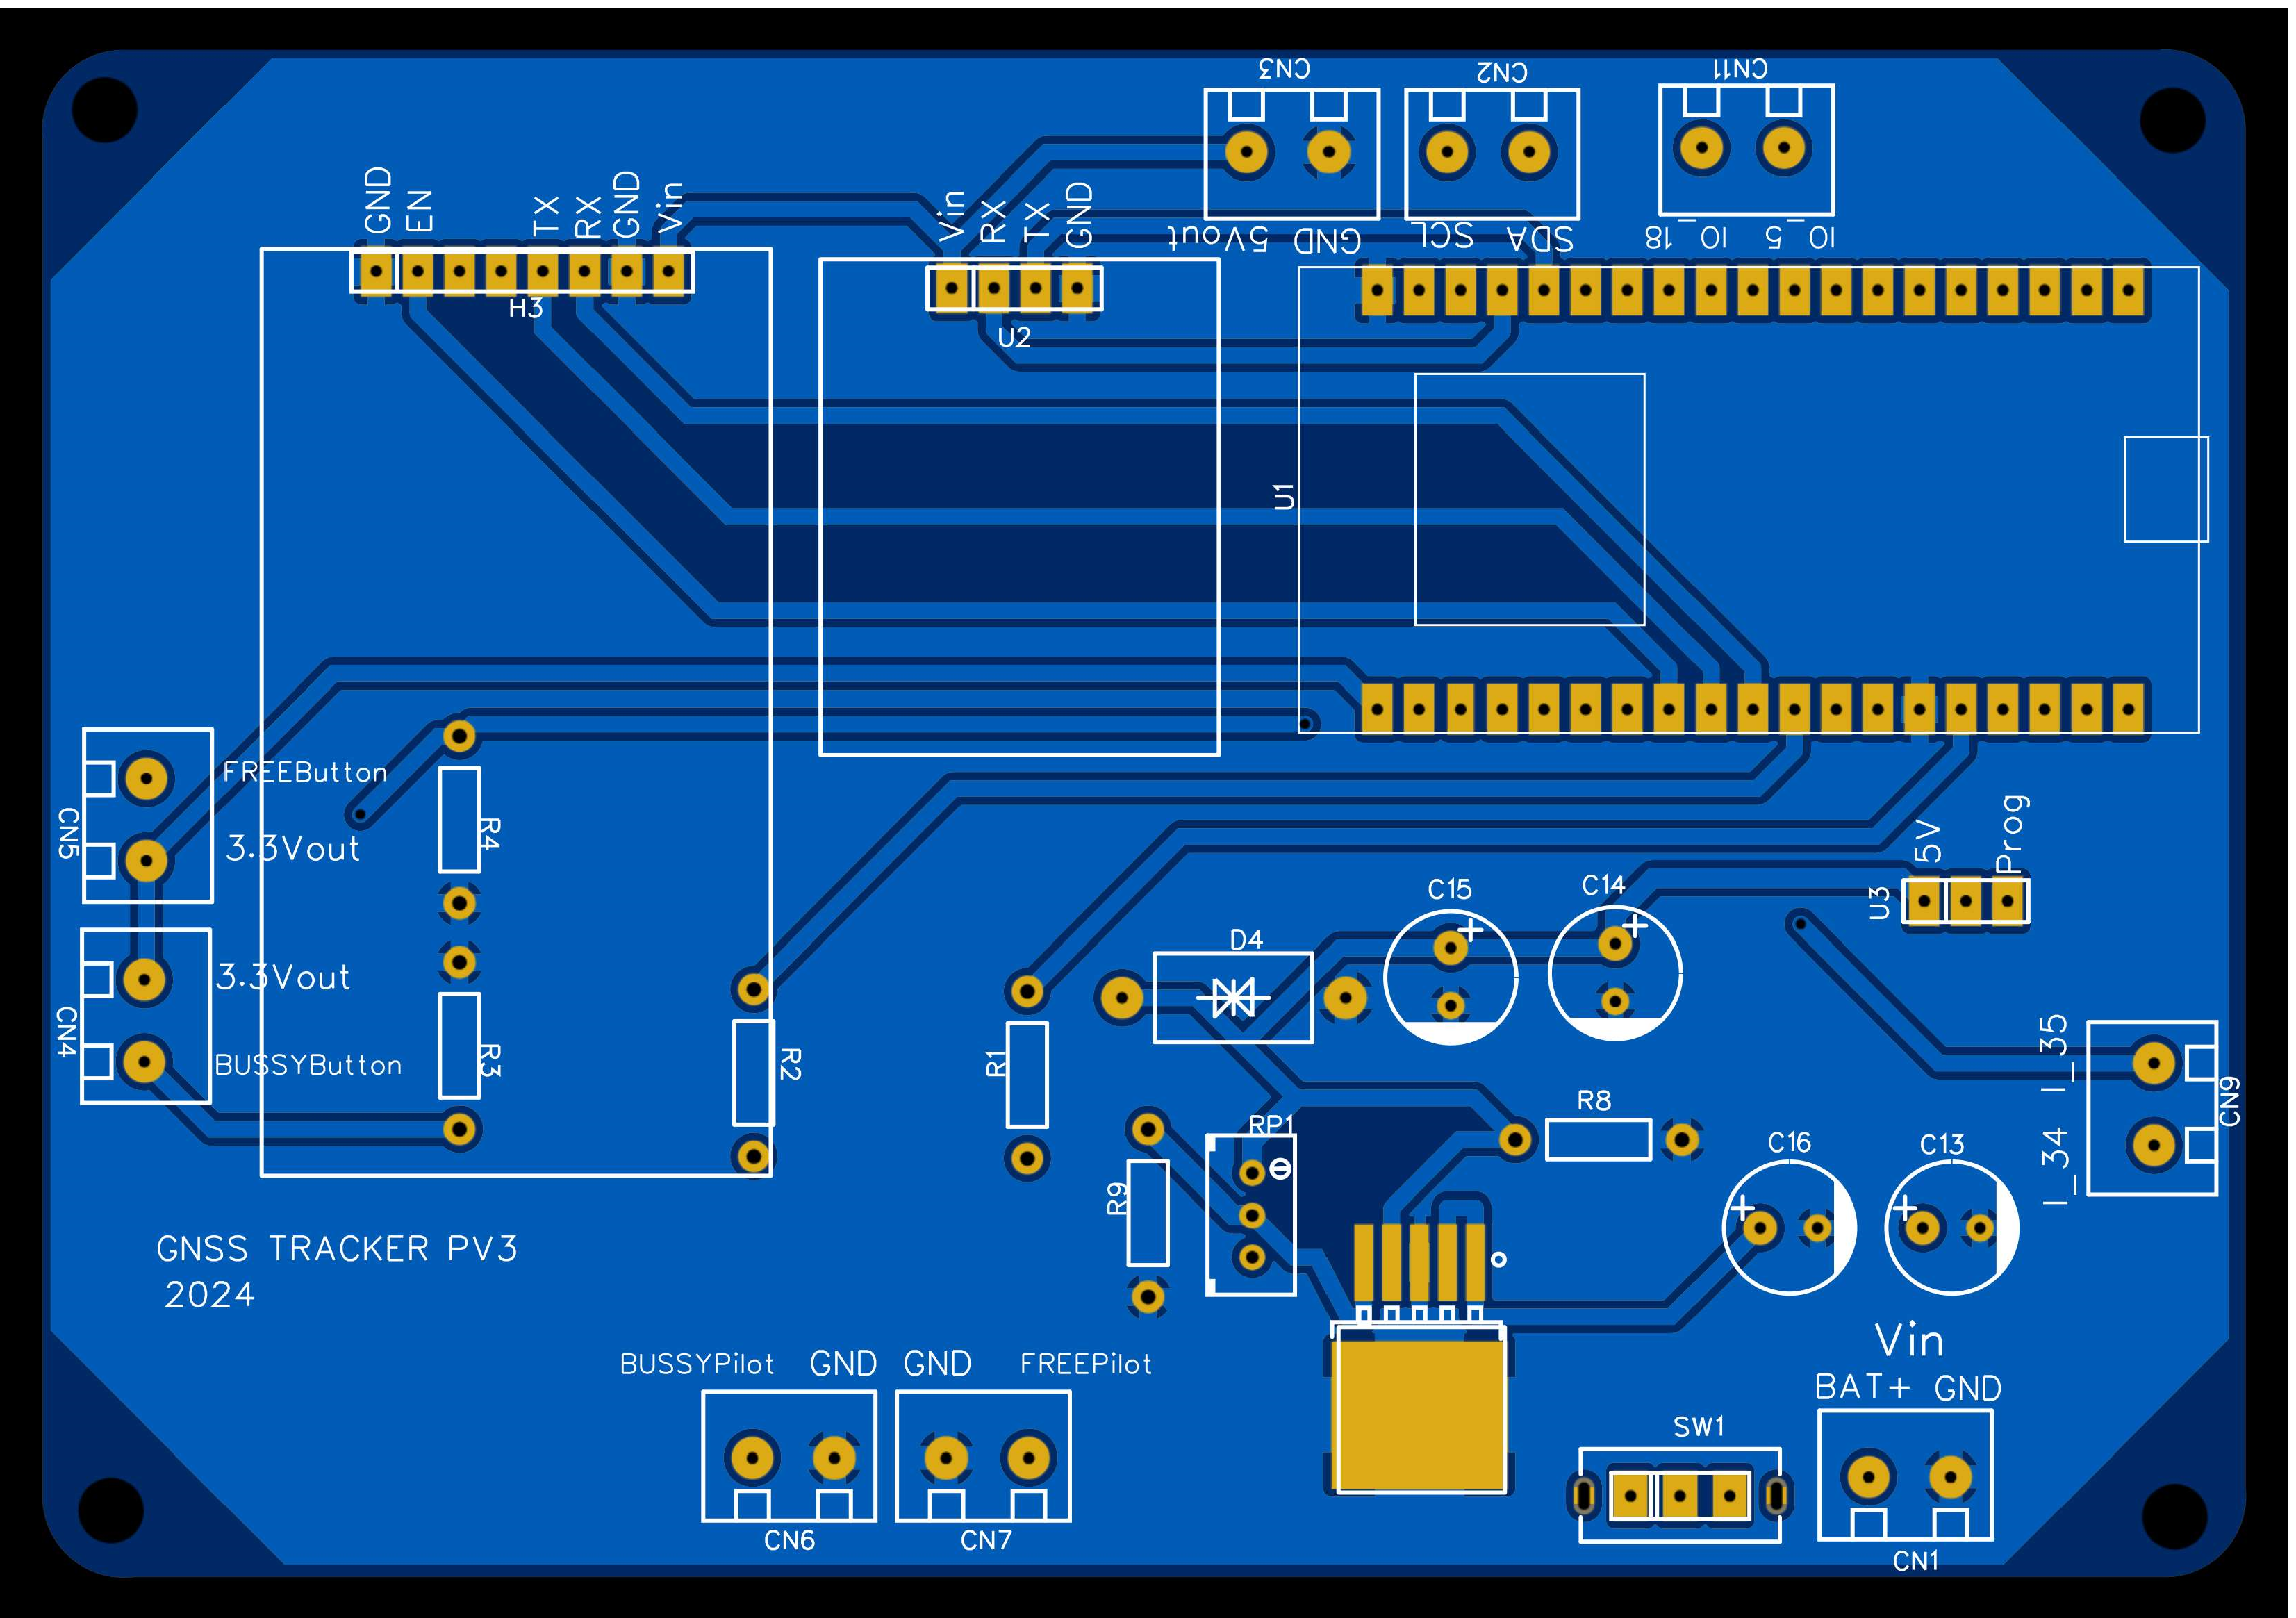
\includegraphics[width=.5\textwidth]{./Figures/PCB_TFE_Modelo_2D.png}
	\caption{Modelo 2D de la placa base del sistema.}
	\label{fig:placa_base_2d}
\end{figure}

\begin{figure}[htbp]
	\centering
	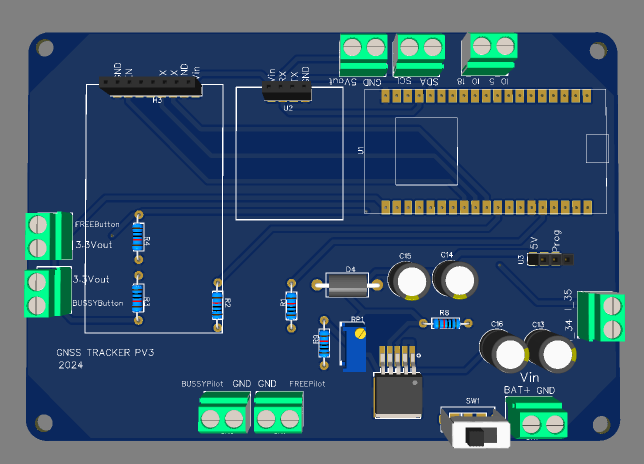
\includegraphics[width=.5\textwidth]{./Figures/PCB_TFE_Modelo_3D.png}
	\caption{Modelo 3D de la placa base del sistema.}
	\label{fig:placa_base_3d}
\end{figure}


\subsubsection{Adaptador para el módulo Quectel L76}

El circuito esquemático del adaptador L76 se encuentra en la figura~\ref{fig:adap_L76}. En este esquemático se puede observar la fuente de 3.3 VDC. Además, en la figura se presenta el circuito de entrada de alimentación, la conexión UART y la conexión entre el módulo y el microcontrolador ESP32.  

En la figura~\ref{fig:adap_L76_3d}, se puede observar el modelo 3D del circuito diseñado. 

\begin{figure}[htbp]
	\centering
	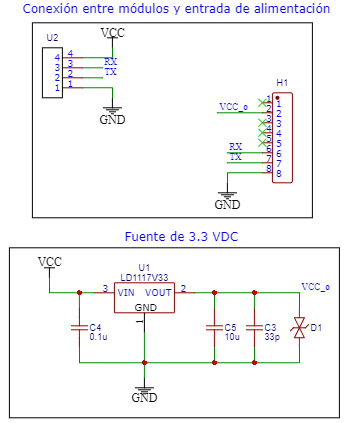
\includegraphics[width=.5\textwidth]{./Figures/QL76_Esquematico.png}
	\caption{Esquemático del adaptador L76.}
	\label{fig:adap_L76}
\end{figure}

\begin{figure}[htbp]
	\centering
	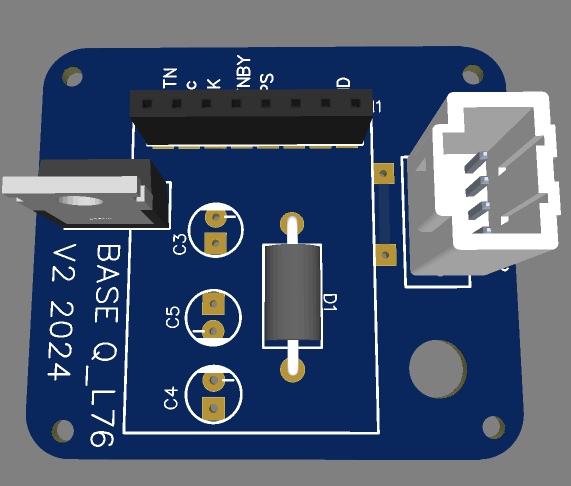
\includegraphics[width=.5\textwidth]{./Figures/QL76_modelo_3d_sup.png}
	\caption{Modelo 3D del adaptador L76.}
	\label{fig:adap_L76_3d}
\end{figure}



%----------------------------------------------------------------------------------------
%	SECTION 3
%----------------------------------------------------------------------------------------
\section{Diseño e implementación del firmware}

En esta sección se presentan las consideraciones de diseño y el proceso de implementación del firmware. 

\subsection{Diseño del firmware}

El propósito del firmware desarrollado es satisfacer los requerimientos de conectividad, administración del hardware e interfaz con el usuario. De acuerdo con esto, a continuación se describen las principales funcionalidades del firmware: 

\begin{enumerate}
 \item Realizar las funciones de conexión a internet a través de la red celular y conexión de área local con wifi. Dentro de estas funciones se encuentran:
 	\begin{enumerate}
 		\item Comunicación a través de comandos AT por el puerto UART con el módulo SIM A7670SA, para asegurar la conexión con el servidor utilizando el protocolo MQTT.
 		\item Utilización del módulo wifi de la ESP32 para generar una conexión wifi cuando exista una red conocida. Transmisión de datos a través del protocolo MQTT. 
 	\end{enumerate}
 \item Comunicación a través de tramas NMEA por el puerto UART con el módulo Quectel L76. Para la recepción e interpretación de la información de geolocalización de las constelaciones GPS y BeiDou.  
 \item Monitoreo de los botones de ocupación a través de interrupciones y visualización de los estados de ocupación a través de los pilotos. 
 \item Generación de interfaz visual a través de la comunicación I2C con la pantalla LCD 16x2. 
 \item Administración de la energía del sistema a través de los modos de bajo consumo de los módulos del sistema. 
 \item Administración de los recursos del microcontrolador a través de la implementación del sitema operativo en tiempo real FreeRTOS. 
\end{enumerate}

\subsubsection{Arquitectura del firmware}
\label{arquitectura_firmware}

De acuerdo con lo planteado anteriormente, en la figura~\ref{fig:arq_firmware} se presenta un diagrama de componentes UML, que representa la arquitectura del sistema. 

\begin{figure}[htbp]
	\centering
	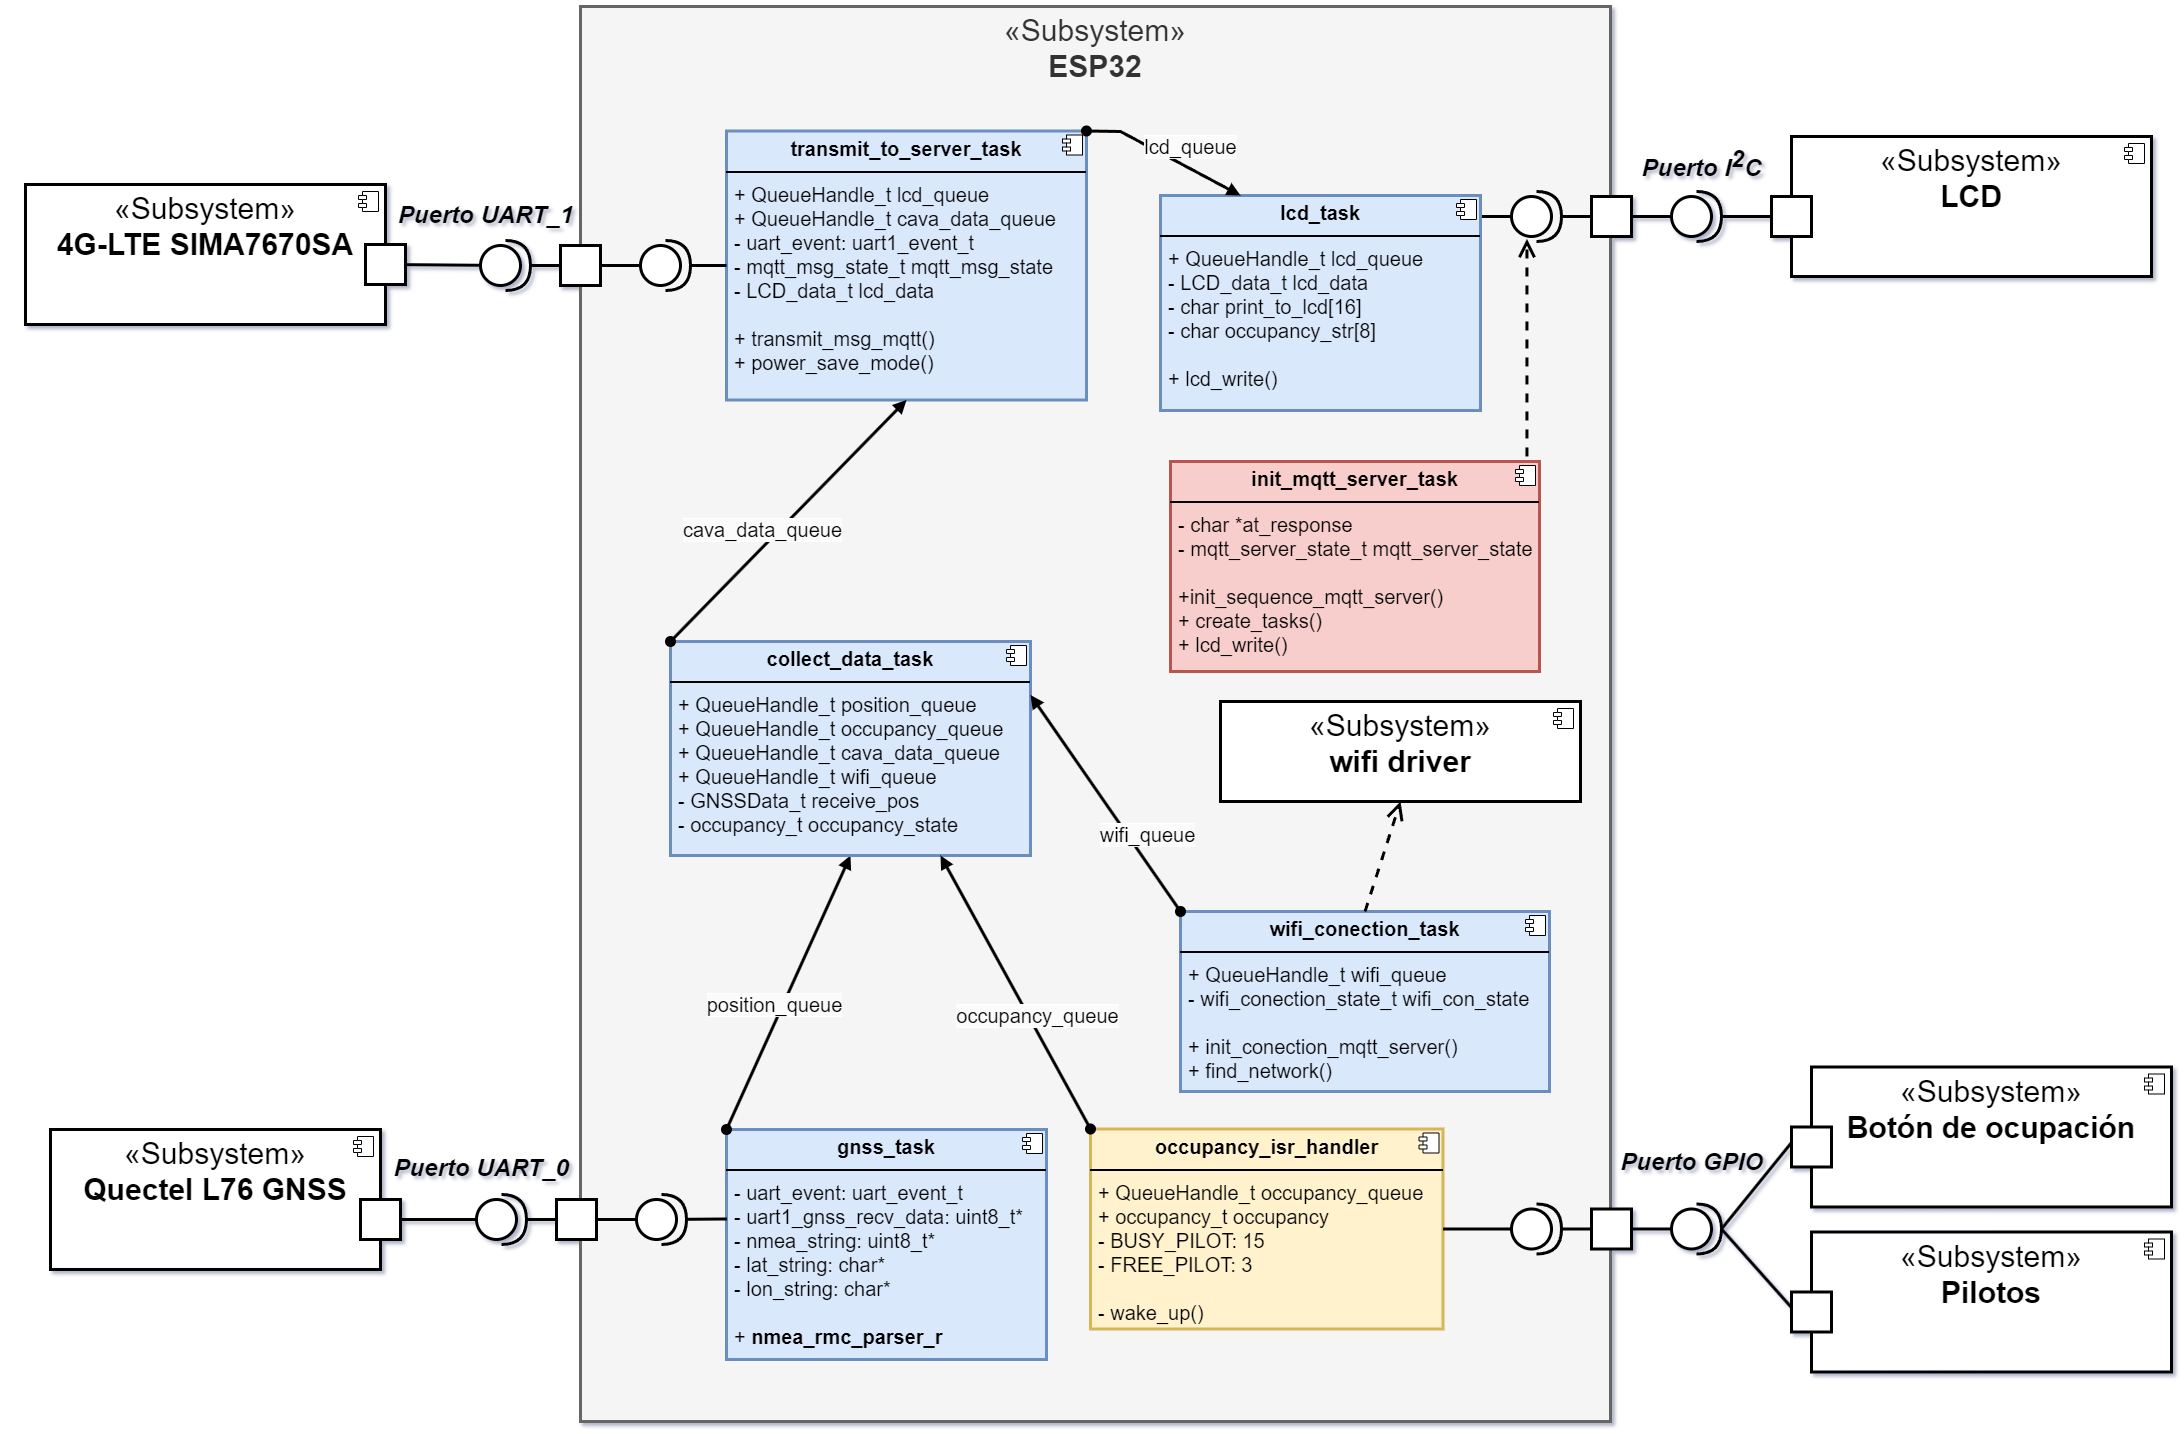
\includegraphics[width=1\textwidth]{./Figures/Arquitectura_firmware_TFE_GNSS.png}
	\caption{Arquitectura del firmware.}
	\label{fig:arq_firmware}
\end{figure}


\subsection{Implementación del firmware}





%----------------------------------------------------------------------------------------
%	SECTION 4
%----------------------------------------------------------------------------------------
\section{Diseño e implementación de la interfaz web}

\subsection{Diseño de la interfaz web}


\subsection{Implementación de la interfaz web}





















\begin{comment}

\definecolor{mygreen}{rgb}{0,0.6,0}
\definecolor{mygray}{rgb}{0.5,0.5,0.5}
\definecolor{mymauve}{rgb}{0.58,0,0.82}

%%%%%%%%%%%%%%%%%%%%%%%%%%%%%%%%%%%%%%%%%%%%%%%%%%%%%%%%%%%%%%%%%%%%%%%%%%%%%
% parámetros para configurar el formato del código en los entornos lstlisting
%%%%%%%%%%%%%%%%%%%%%%%%%%%%%%%%%%%%%%%%%%%%%%%%%%%%%%%%%%%%%%%%%%%%%%%%%%%%%
\lstset{ %
  backgroundcolor=\color{white},   % choose the background color; you must add \usepackage{color} or \usepackage{xcolor}
  basicstyle=\footnotesize,        % the size of the fonts that are used for the code
  breakatwhitespace=false,         % sets if automatic breaks should only happen at whitespace
  breaklines=true,                 % sets automatic line breaking
  captionpos=b,                    % sets the caption-position to bottom
  commentstyle=\color{mygreen},    % comment style
  deletekeywords={...},            % if you want to delete keywords from the given language
  %escapeinside={\%*}{*)},          % if you want to add LaTeX within your code
  %extendedchars=true,              % lets you use non-ASCII characters; for 8-bits encodings only, does not work with UTF-8
  %frame=single,	                % adds a frame around the code
  keepspaces=true,                 % keeps spaces in text, useful for keeping indentation of code (possibly needs columns=flexible)
  keywordstyle=\color{blue},       % keyword style
  language=[ANSI]C,                % the language of the code
  %otherkeywords={*,...},           % if you want to add more keywords to the set
  numbers=left,                    % where to put the line-numbers; possible values are (none, left, right)
  numbersep=5pt,                   % how far the line-numbers are from the code
  numberstyle=\tiny\color{mygray}, % the style that is used for the line-numbers
  rulecolor=\color{black},         % if not set, the frame-color may be changed on line-breaks within not-black text (e.g. comments (green here))
  showspaces=false,                % show spaces everywhere adding particular underscores; it overrides 'showstringspaces'
  showstringspaces=false,          % underline spaces within strings only
  showtabs=false,                  % show tabs within strings adding particular underscores
  stepnumber=1,                    % the step between two line-numbers. If it's 1, each line will be numbered
  stringstyle=\color{mymauve},     % string literal style
  tabsize=2,	                   % sets default tabsize to 2 spaces
  title=\lstname,                  % show the filename of files included with \lstinputlisting; also try caption instead of title
  morecomment=[s]{/*}{*/}
}

Se puede agregar código o pseudocódigo dentro de un entorno lstlisting con el siguiente código:

\begin{verbatim}
\begin{lstlisting}[caption= "un epígrafe descriptivo"]
	las líneas de código irían aquí...
\end{lstlisting}
\end{verbatim}

A modo de ejemplo:

\begin{lstlisting}[label=cod:vControl,caption=Pseudocódigo del lazo principal de control.]  % Start your code-block

#define MAX_SENSOR_NUMBER 3
#define MAX_ALARM_NUMBER  6
#define MAX_ACTUATOR_NUMBER 6

uint32_t sensorValue[MAX_SENSOR_NUMBER];		
FunctionalState alarmControl[MAX_ALARM_NUMBER];	//ENABLE or DISABLE
state_t alarmState[MAX_ALARM_NUMBER];						//ON or OFF
state_t actuatorState[MAX_ACTUATOR_NUMBER];			//ON or OFF

void vControl() {

	initGlobalVariables();
	
	period = 500 ms;
		
	while(1) {

		ticks = xTaskGetTickCount();
		
		updateSensors();
		
		updateAlarms();
		
		controlActuators();
		
		vTaskDelayUntil(&ticks, period);
	}
}
\end{lstlisting}

\end{comment}

